Per lo studio delle geometrie molecolari utilizzeremo due approcci diversi: prima tratteremo delle molecole semplici, dopodiché vedremo come sia possibie generalizzare alcune informazioni per studiare molecole più complesse.
\subsection{Lo stato di promozione del carbonio}
Consideriamo la molecola del metano \ce{CH_4}. In essa il carbonio è legato a quattro atomi di idrogeno, per cui la sua valenza è pari a 4.

La configurazione elettronica del carbonio nello stato fondamentale però è
$$\text{C} \quad 1s^22s^22p_x^12p_y^12p_z^0 \quad \subshell{1s:2} \; \subshell{2s:2} \; \subshell{2p:110}$$
Nota: l'avere scritto  un elettrone nel 2p$_x$, uno nel 2p$_y$ e zero nel 2p$_z$ è stata una nostra scelta: potevamo scegliere che fosse vuoto il 2p$_x$ e occupati 2p$_y$ e 2p$_z$, oppure che fosse vuoto il 2p$_y$ e occupati 2p$_x$ e 2p$_z$

Avendo solo due orbitali parzialmente occupati, questa configurazione ci porta a pensare che il carbonio abbia valenza 2, in contrasto in quasi tutti i suoi composti il carbonio è tetravalente.

Per spiegare la valenza 4, si è pensato che uno degli elettroni degli orbitali 2s (che col 2p sono i livelli di valenza) possa essere promosso al restante orbitale p vuoto in modo tale che la confogurazione elettronica del carbonio in questo nuovo stato, detto di promozione, sia

$$\text{C} \quad 1s^22s^12p_x^12p_y^12p_z^1 \quad \subshell{1s:2} \; \subshell{2s:1} \; \subshell{2p:111}$$
Vedremo che questa teoria riuscirà a spiegare anche la valenza di elementi in composti non organici.

Lo stato di promozione tuttavia riesce a giustificare solo la valenza 4 del carbonio, ma non la geometria del metano: sperimentalmente per esso si misurano quattro legami tutti uguali, ma se abbiamo pensato di avere parzialmente occupati un orbitale s e tre orbitali p non ce li aspetteremmo tali, in quanto gli orbitali p sono direzionali (in particolar modo sono diretti lungo gli assi cartesiani), mentre l'orbitale s è a simmetria sferica. Inoltre i legami dovuti ai tre orbitali p dovrebbero stare a 90° l'uno dall'altro, ma nei fatti gli angoli sono di 109.5°.
\subsection{L'ibridizzazione sp$^3$}
A questo punto interviene la teoria dell'ibridizzazione, ossia si parla di \textbf{orbitali ibridi} sp: si pensa che i tre orbitali p e l'orbitale s si mescolino fra loro per dare luogo a quattro orbitali identici, a meno della diversa orientazione, i quali si chiamanno ibridi proprio perché hanno sia carattere s che carattere p.

Gli orbitali sp possiedono un lobo molto più grande dell'altro, ciò è dovuto al fatto che le funzioni d'onda degli orbitali p hanno un segno che segue quello dell'asse lungo cui sono orientati, e in particolare hanno un lobo sul semiasse positivo e uno sul semiasse negativo. Quando li combiniano al 2s che è assunto positivo, avremo una somma per il lobo positivo e una differenza per il quello negativo, da cui segue un rafforzamento della funzione lungo la parte positiva e un decremento lungo quella negativa. Spesso addirittura il lobo piccolo viene trascurato. Inoltre, per comprendere meglio l'orientazione di questi orbitali, il lobo lungo la parte positiva dell'asse viene stilizzato come una goccia allungata:

\begin{figure}[htp]
    \centering
    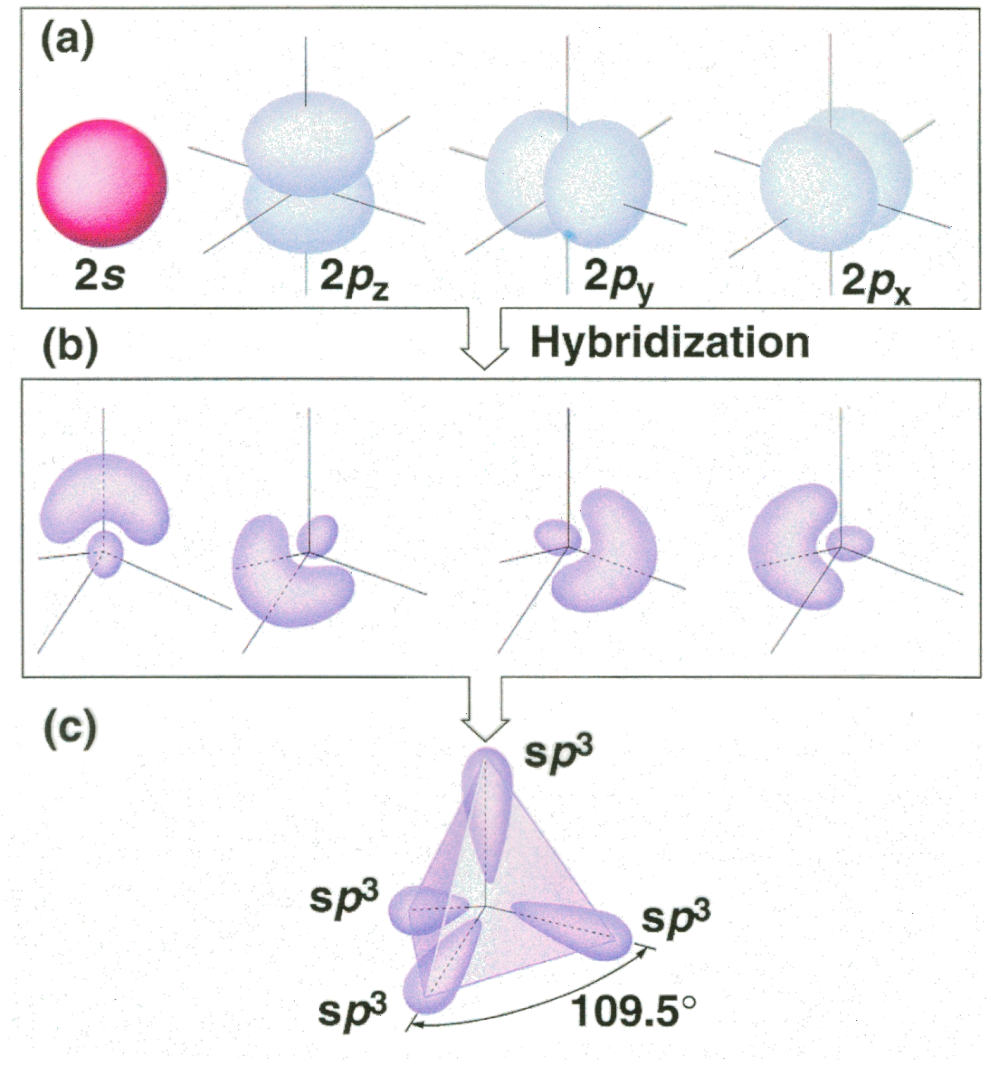
\includegraphics[width=11cm]{immagini/orbitali-sp3.png}
\end{figure}
\newpage
Stilizzandoli diventa evidente che gli orbitali ibridi del carbonio sono orientati lungo i vertici di un tetraedro in cui al centro viene posto il carbonio con i suoi 4 orbitali, i quali formano angoli di 109.5° tra loro. Si può inoltre mostrare che il tetraedro può essere inscritto in un cubo, in cui due vertici del tetraedro coincidono con due vertici della faccia superiore del cubo e gli altri due con i vertici opposti della faccia inferiore. Su ogni vertice ci sarà un idrogeno, mentre il carbonio sarà al centro. Questo è il motivo per cui il tetraedro è etichettato "solido cubico".

Avendo mescolato 4 orbitali atomici, ci aspettiamo 4 orbitali ibridi, che nei fatti osserviamo. Essi si chiamano ibridi sp$^3$, dove il 3 indica il numero di orbitali p e non il loro riempimento. 

Con questa teoria dell'ibridazione riusciamo a giustificare la geometria del metano in quanto ognuno di questi orbitali, su cui è presente un elettrone, interagirà con l'elettrone di un atomo di idrogeno, creando quattro legame identici.\\

La funzione d'onda generica per un generico orbitale ibrido sp$^3$ è

$$\Psi_{sp^3}=c_1\Psi_{2s} + c_2\Psi_{2p_x} + c_3\Psi_{2p_y} + c_4\Psi_{2p_z}$$

dove $c_1$, $c_2$, $c_3$ e $c_4$ sono i pesi di ciascuna funzione, che indicano quanto siano coinvolte le funzioni d'onda in quell'orbitale.

Le equazioni in totale sono 4.

Avendo nei fatti un livello s si mescola con tre orbitali p in egual maniera in quattro funzioni diverse, ognuna di queste conterrà un quarto di carattere s e tre quarti di carattere p.

Le quattro equazioni sono
$$sp_a^3=\frac{1}{2}(s + p_x + p_y + p_z) \qquad sp_b^3=\frac{1}{2}(s - p_x - p_y + p_z)$$
$$sp_c^3=\frac{1}{2}(s + p_x - p_y - p_z) \qquad sp_d^3=\frac{1}{2}(s - p_x + p_y - p_z)$$
Il valore 1/2 è il "coefficiente di normalizzazione", esso fa sì che l'integrale della $\Psi^2$ sia pari a 1.

Consideriamo adesso la molecola dell'etano \ce{C_2H_6}. In entrambi gli atomi di carbonio si ha ibridizzazione sp$^3$, quindi entrambi avranno quattro orbitali ibridi orientati lungo i vertici di un tetraedro
\begin{figure}[htp]
    \centering
    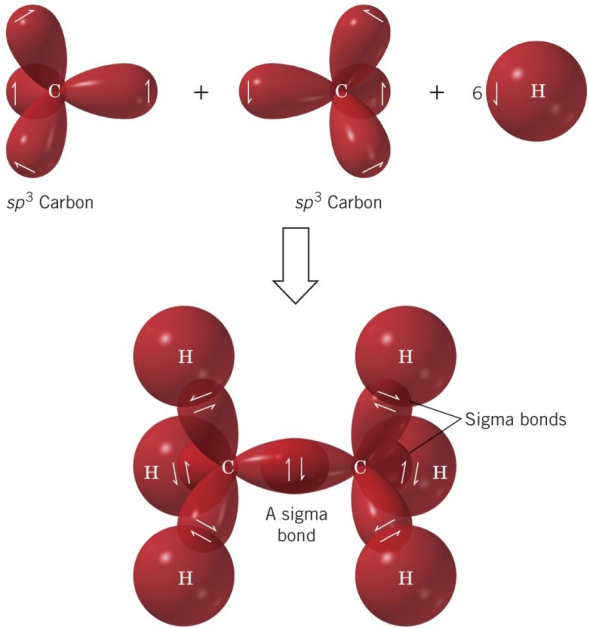
\includegraphics[width=7cm]{immagini/etano.png}
\end{figure}
In modo arbitrario si sceglie quale sia l'asse di legame, cioè quello lungo cui sono legati i due atomi di carbonio, ad esempio l'asse z. Allora i due orbitali ibridi orientati lungo l'asse z, uno per ciascun atomo, interagiranno fra loro accoppiando due elettroni per formare il legame carbonio-carbonio. A questo punto restano 6 orbitali ibridi, ciascuno con un elettrone, e ognuno di questi interagisce con un idrogeno, dando luogo alla molecola di sopra.

Secondo questa teoria la geometria di tale molecola sarebbe quindi quella di due tetraedri collegati tramite un vertice. Nei fatti si osserva proprio questo.

La teoria dell'ibridazione sp$^3$ riesce a spiegare le geometrie di tutti gli alcheni successivi (butano, propano, pentano ecc.)

\subsection{Ibridizzazione sp$^2$}
Immaginiamo ora che solo 2 orbitali p si mescolino con l'orbitale s, mentre il terzo resti rigorosamente atomico. In questo modo vengono fuori tre orbitali ibridi detti sp$^2$.

Le molecole in cui il carbonio mostra questo tipo di ibridazione sono planari, cioè gli orbitali giacciono tutti sullo stesso piano e se stilizziamo gli orbitali ci accorgiamo che questi puntano a 120° l'uno dall'altro. Si dice che hanno geometria "trigonale planare". Inoltre, perpendicolarmente a questo piano, abbiamo un orbitale p non coinvolto nell'ibridizzazione, il quale però mantiene un elettrone (vale ancora il discorso dello stato di promozione, altrimenti non potremmo spiegare la tetravalenza)

\begin{figure}[htp]
    \centering
    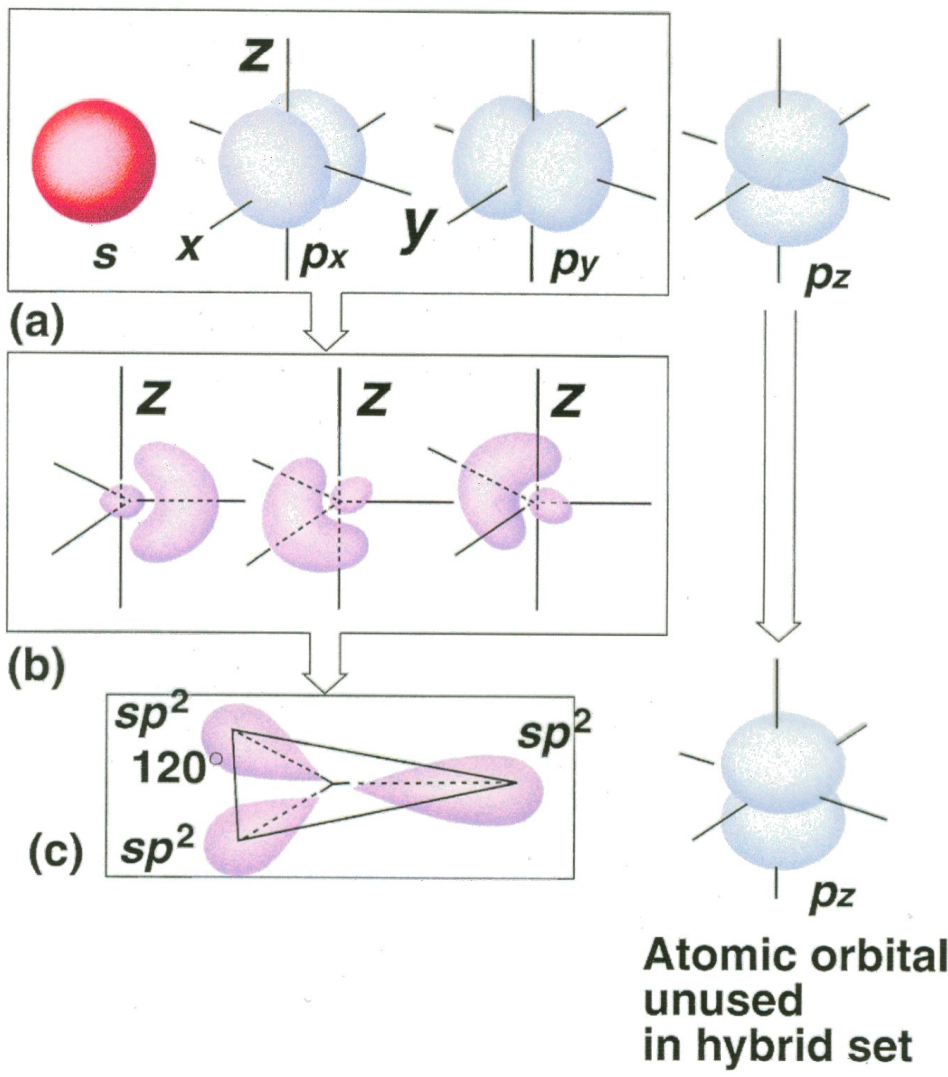
\includegraphics[width=11cm]{immagini/orbitali-sp2.png}
\end{figure}

Consideriamo ora la configurazione elettronica del boro:
$$\text{B} \quad 1s^22s^22p_x^12p_y^02p_z^0 \quad \subshell{1s:2} \; \subshell{2s:2} \; \subshell{2p:100}$$
Per giustificare la valenza 3 del boro immaginiamo che un elettrone dell'orbitale 2s venga promosso ad uno dei tre orbitali p, in modo da avere tre orbitali parzialmente occupati: 
$$\text{B} \quad 1s^22s^12p_x^12p_y^12p_z^0 \quad \subshell{1s:2} \; \subshell{2s:1} \; \subshell{2p:110}
$$
Se questi si mescolano fra loro per dar luogo ad ibridi sp$^2$, ci attendiamo molecole planari trigonali. Anche qui avremo un orbitale p puro perpendicolare al piano della molecola, solo che stavolta sarà vuoto.

Se osserviamo la molecola trifluoruro di boro \ce{BF_3}, essa ha proprio questa geometria. Inoltre il fluoro è l'elemento più elettronegativo, quindi la differenza in elettronegatività tra fluoro e boro è alta, motivo per cui ci aspettiamo che la carica degli elettroni di legame sia fortemente attratta dal fuoro che quindi si negativizza, mentre il boro si positivizza. Ne segue che ogni legame boro-fluoro costituirà un dipolo. Tuttavia, grazie alla struttura planare della molecola, in cui gli angoli sono tutti uguali, la somma dei momenti di dipolo è nulla. Se il boro non fosse stato sul piano la molecola avrebbe avuto un momento di dipolo risultante.\\

Gli orbitali ibridi sp$^2$ sono tre, quindi stavolta essi avranno un terzo di carattere s e due terzi di carattere p.

La generica equazione di un tale orbitale ibridi avrà una forma del tipo

$$\Psi_{sp^2}=c_1\Psi_{2s} + c_2\Psi_{2p_x} + c_3\Psi_{2p_y}$$
$$sp^2_a=\frac{1}{\sqrt{3}}\Biggl(s + \sqrt{2}p_x\Biggr)
$$
$$
sp^2_b=\frac{1}{\sqrt{3}}\left(s - \frac{\sqrt{3}}{\sqrt{6}}p_x +\frac{\sqrt{3}}{\sqrt{2}}p_y\right)
$$
$$
sp^2_c=\frac{1}{\sqrt{3}}\left(s - \frac{\sqrt{3}}{\sqrt{6}}p_x + \frac{\sqrt{3}}{\sqrt{2}}p_y\right)
$$

Questo tipo di ibridazione permette di spiegare anche la geometria di tutti gli alcheni, composti del carbonio in cui è presente un doppio legame carbonio-carbonio. Il primo di questi è l'acetilene o etene \ce{C_2H_4}, in cui i due atomi di carbonio hanno ibridazione sp$^2$. In entrambi gli atomi uno dei tre orbitali ibridi viene usato per fare il legame carbonio-carbonio, gli altri due per legare gli idrogeni. Ci aspettiamo che il sistema \ce{CH_2-CH_2} sia planare, ed è così: i due carbonio e i quattro idrogeni stanno tutti sullo stesso piano, e gli angoli di legame sono di 120°.

Ragioniamo adesso sui due orbitali p non coinvolti nell'ibridazione: essi sono perpendicolari al piano della molecola e hanno ciascuno un elettrone. Se orientiamo questi orbitali (ricordiamo che gli orbitali p hanno un segno) in modo che abbiano lo stesso segno, si avrà che questi orbitali interagiranno sopra e sotto il piano della molecola e daranno luogo ad un secondo legame carbonio-carbonio che sarà di tipo $\pi$ in quanto la densità di carica non sarà lungo l'asse di legame come nel caso del legame $\sigma$, ma sopra e sotto.

\begin{figure}[htp]
    \centering
    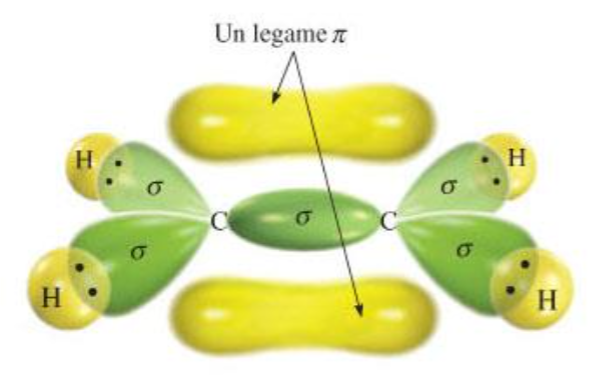
\includegraphics[width=11cm]{immagini/etene.png}
\end{figure}

Va da notare che tutti i legami dovuti agli ibridi sono sempre legami $\sigma$, perché diretti lungo la congiungente dei nuclei, quindi non ci sono nodi lungo gli assi di legame tra carbonio e idrogeno o tra carbonio e carbonio, o tra gli altri elementi che abbiamo visto. I legami che invece creano gli orbitali p non ibridizzati non giacciono sul piano, e il motivo è che lungo il piano essi hanno un nodo.

Attenzione! Se essi avessero puntato coi lobi l'uno contro l'altro avremmo ottenuto comunque un legame $\sigma$\\

Consideriamo infine il benzene \ce{C_6H_6}. Esso è un composto del carbonio avente struttura planare a forma di esagono regolare, dove ogni vertice rappresenta un gruppo CH. Essendo planare, il carbonio ha ibridazione sp$^2$ e quindi ha tre orbitali ibridi, di cui uno viene usato per formare il legame carbonio-idrogeno, gli altri due per formare i legami carbonio-carbonio da un lato e dall'altro. L'insieme di questi legami lungo il piano costituisce lo "scheletro $\sigma$" della molecola

Ogni atomo manterrà poi un orbitale p puro perpendicolare al piano, il quale ha un elettrone disponibile a formare un legame. In totale avremo quindi 6 elettroni, che danno luogo a tre legami $\pi$, che vengono rappresentati con dei doppi legami alternati:
$$
\schemestart
\chemfig{*6(=-=-=-=)}
\arrow{<->}
\chemfig{*6(-=-=-=)}
\schemestop
$$
Non c'è un motivo per cui i doppi legami debbano essere posizionati come a sinistra o come a destra, cioè non c'è un motivo per cui scrivere una formula anziché l'altra: sono due formule limite.

Nella realtà tutti e sei gli atomi godono di un parziale doppio legame, cioè i tre doppi legami si ripartiscono su sei legami, per cui non avremo tre legami con ordine di legame 1 e tre con ordine di legame 2, ma avranno tutti ordine 1.5. Per indicare ciò si preferisce disegnare un anello all'interno dell'esagono

%\begin{figure}[htp]
%    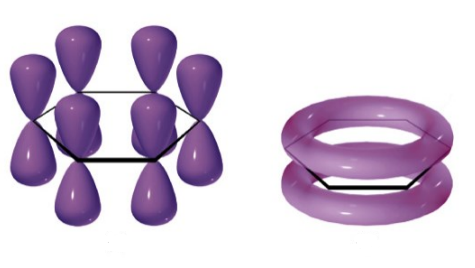
\includegraphics[width=8cm]{immagini/benzene.png}
%\end{figure}

\chemfig{**6(------)}\

\subsection{Ibridizzazione sp}
Immaginiamo di mescolare sono uno dei tre orbitali 2p con l'orbitale 2s: otterremo due orbitali ibridi sp. Essi, se stilizzati, mostrano che i lobi giacciono su una linea, quindi tra loro gli angoli sono di 180°. Dunque la geometria è lineare.

I due orbitali p non ibridizzati saranno perendicolari all'asse, che conterranno un elettrone ciascuno nel caso del carbonio

\begin{figure}[htp]
    \centering
    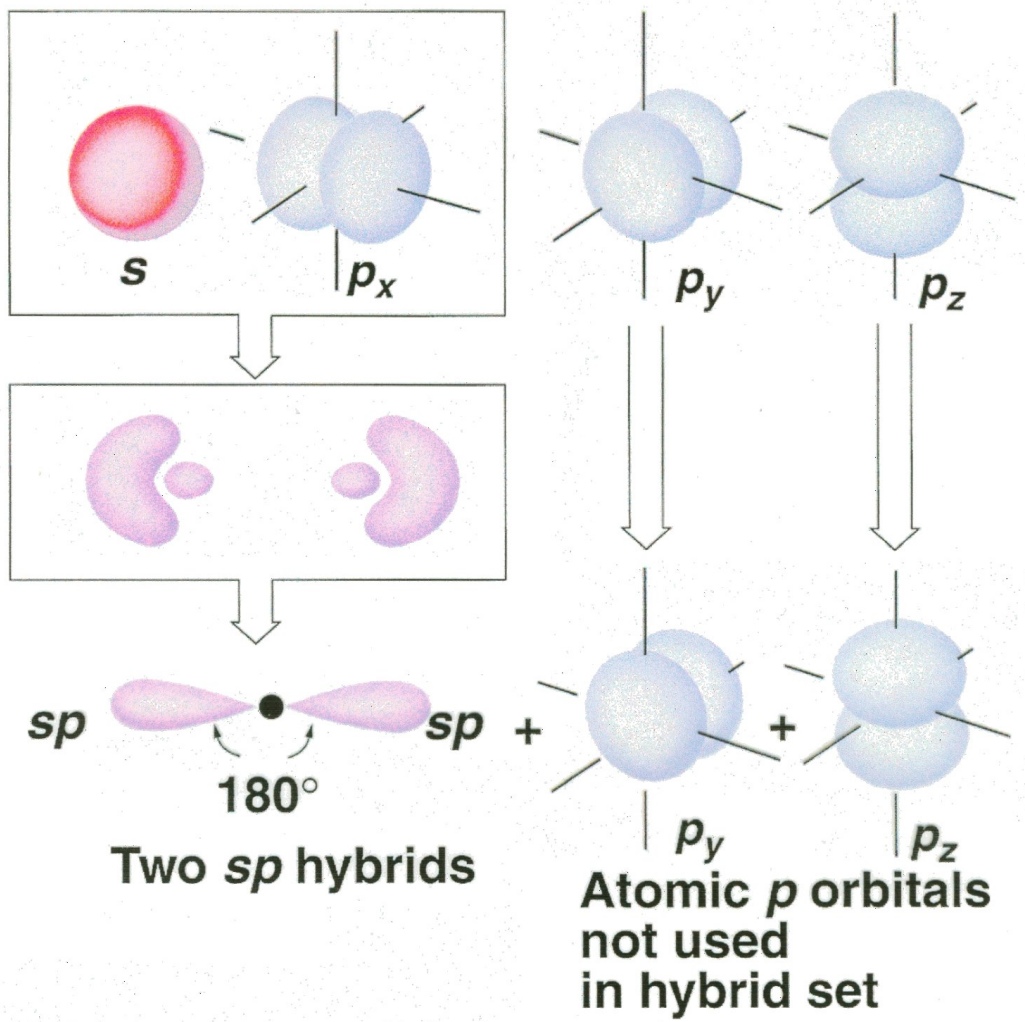
\includegraphics[width=9cm]{immagini/orbitali-sp.png}
\end{figure}
Stavolta un orbitale s e uno p si ripartiscono in due orbitali, quindi questi avranno metà carattere s e metà carattere p:
$$\Psi_{sp}= c_1\Psi_{2s} + c_2\Psi{2p}$$
$$
sp_a=\frac{1}{\sqrt{2}}(s + p_x)
\qquad
sp_b=\frac{1}{\sqrt{2}}(s - p_x)
$$
Tale ibridazione permette di spiegare la geometria degli alchini, composti in cui è presente un triplo legame carbonio-carbonio, come ad esempio l'acetilene \ce{C_2H_2}. In essa un orbitale ibrido viene usato per creare il legame carbonio-carbonio, l'altro il legame carbonio-idrogeno. Abbiamo poi due orbitali p non ibridizzati su ciascun atomo di carbonio, i quali reagiscono a coppie per dare luogo a due legami $\pi$, a 90° l'uno dall'altro:
\begin{figure}[htp]
    \centering
    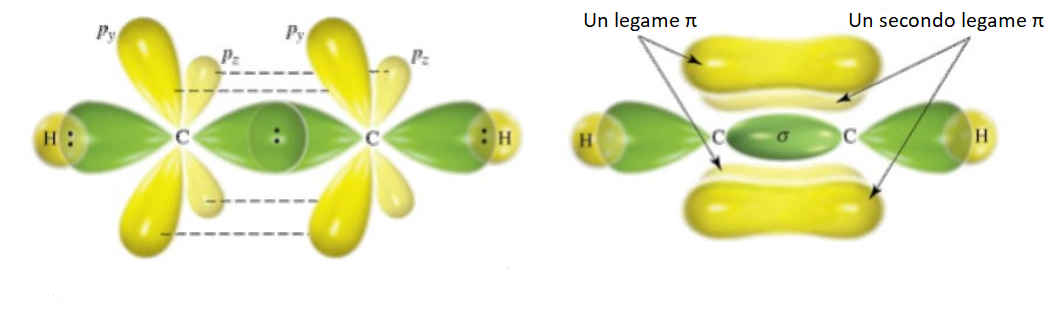
\includegraphics[width=14cm]{immagini/acetilene.png}
\end{figure}
Consideriamo la configurazione elettronica del berillio:
$$\text{Be} \quad 1s^22s^22p_x^02p_y^02p_z^0 \quad \subshell{1s:2} \; \subshell{2s:2} \; \subshell{2p:000}$$
Per spiegare la valenza 2, immaginiamo che un elettrone del 2s venga promosso ad un orbitale 2p, ottenendo così due orbitali parzialmente occupati:
$$\text{Be} \quad 1s^22s^12p_x^12p_y^02p_z^0 \quad \subshell{1s:2} \; \subshell{2s:1} \; \subshell{2p:100}$$
A questo punto pensiamo che l'orbitale s si mescoli con un orbitale p per dare luogo a due orbitali sp. In questo caso i due orbitali p non ibridizzati saranno vuoti. 

Se osserviamo la molecola del cloruro di berillio \ce{BeCl_2}, essa ha una geometria lineare.\\

